\chapter{The Sample Kits}


\xentrystretch{-0.05}
\tablehead{%
%\hline
\multicolumn{1}{l}{\bf{Machine}} &
\multicolumn{1}{l}{\bf{Year}} &
\multicolumn{1}{l}{\bf{Info}}
\\
}
%\tabletail{ \hline }
\tablelasttail{ \hline }
%\tablelasttail{ \multicolumn{3}{l}{} \\ \hline }
\begin{xtabular}{p{2.4cm}|l|p{9.1cm}}

\hline
SP0256-AL2 \linebreak
General Instruments 
& 1981 & 
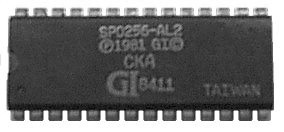
\includegraphics[width=5.6cm]{sp0256al2}

The SP0256-AL2 Speech Processor IC contains a programmable digital filter that can be made to model a vocal tract. The 16k ROM stores both data and instructions. The pulse width modulated output can produce speech with a frequency range of 5kHz and a dynamic range of 42 dB. \\
\hline
TR-606 \linebreak Roland & 1981 & 
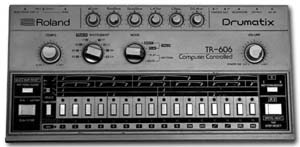
\includegraphics[width=7cm]{tr606}

The Roland TR-606 Drumatix is a programmable analogue drum machine. It was designed to couple with the TB-303 Bassline. The TR-606 has a very original sound and remains popular today. \\
\hline
TR-707 \linebreak Roland & 1984 & 
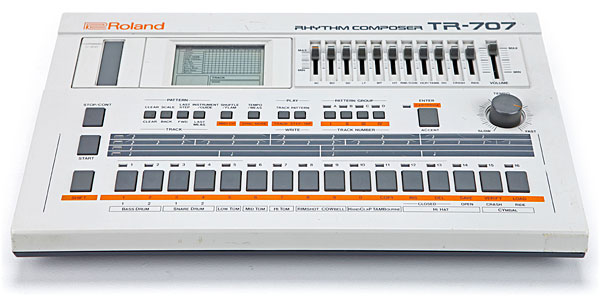
\includegraphics[width=6.9cm]{tr707}

The Roland TR-707 has the same functions as the TR-909 with all PCM sounds. Starting with this model, Roland began using an LCD display to show the rhythm matrix and tempo. \\
\hline
TR-727 \linebreak Roland & 1985 & 
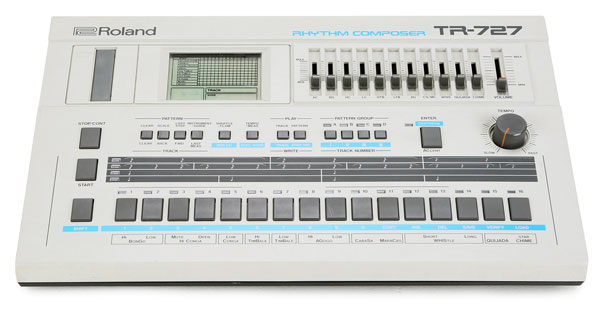
\includegraphics[width=6.9cm]{tr727}

The Roland TR-727 is identical to the TR-707, with the exception that its sounds are Ethnic/Latin percussion. It is meant to complement a rhythm section, rather than be a main unit. \\
\hline
TR-808 \linebreak Roland & 1980 & 
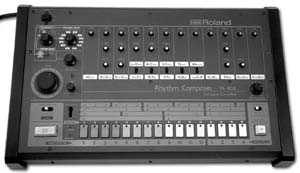
\includegraphics[width=8.4cm]{tr808}

The Roland TR-808 has played a defining role for the 80's Hip Hop and Electro movement. It is still highly popular, thanks to its unmistakably original sounds. \\
\hline
TR-909 \linebreak Roland & 1983 & 
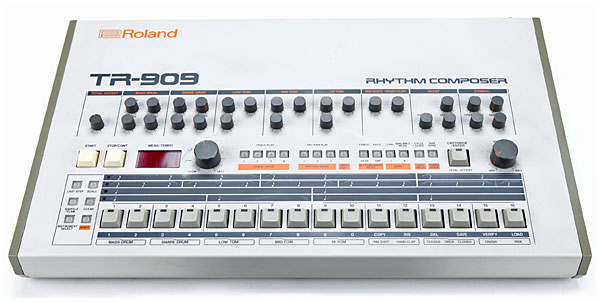
\includegraphics[width=6cm]{tr909}

The Roland TR-909 is one of the most popular drum machines ever. It has PCM sounds for cymbal and hi-hat, but all other instruments still come from analogue circuitry. The sounds are very useful for House and Techno music. \\
\hline
CR-78 \linebreak Roland & 1978 & 
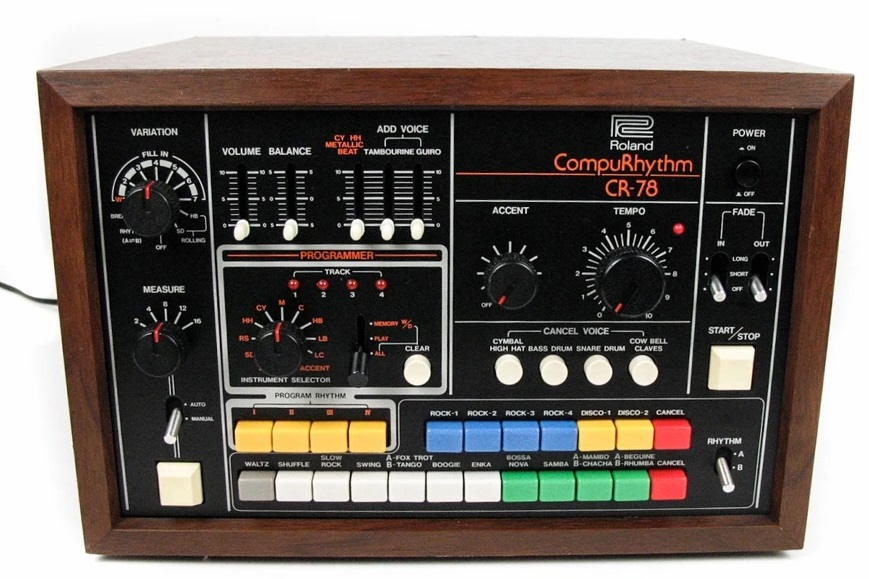
\includegraphics[width=6cm]{cr78}

The Roland CR-78 is perhaps the most luxurious rhythm machine ever made. The guiro and tambourine are still unique as of today, and bass, snare and bongos sound very soft and rich. \\
\hline
CR-8000 \linebreak Roland & 1981 & 
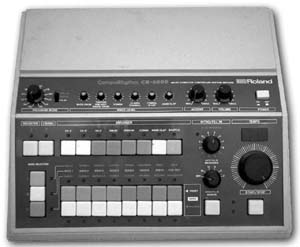
\includegraphics[width=6cm]{cr8000}

The Roland CR-8000 was introduced after the TR-808 -- it has the same analog engine. The hi-hat sounds more realistic than older rhythm machines, but the hand clap sounds like an electric snare. \\
\hline
DR-55 \linebreak Boss & 1979 & 
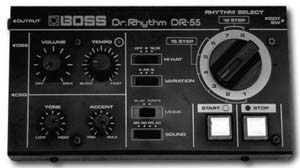
\includegraphics[width=6.9cm]{dr55}

The Boss Dr. Rhythm range of drum machines is especially designed for guitar players who need a mobile drummer. The DR-55 is a simple analogue drum machine with a very rough and direct sound. \\
\hline
DR-110 \linebreak Boss & 1983 & 
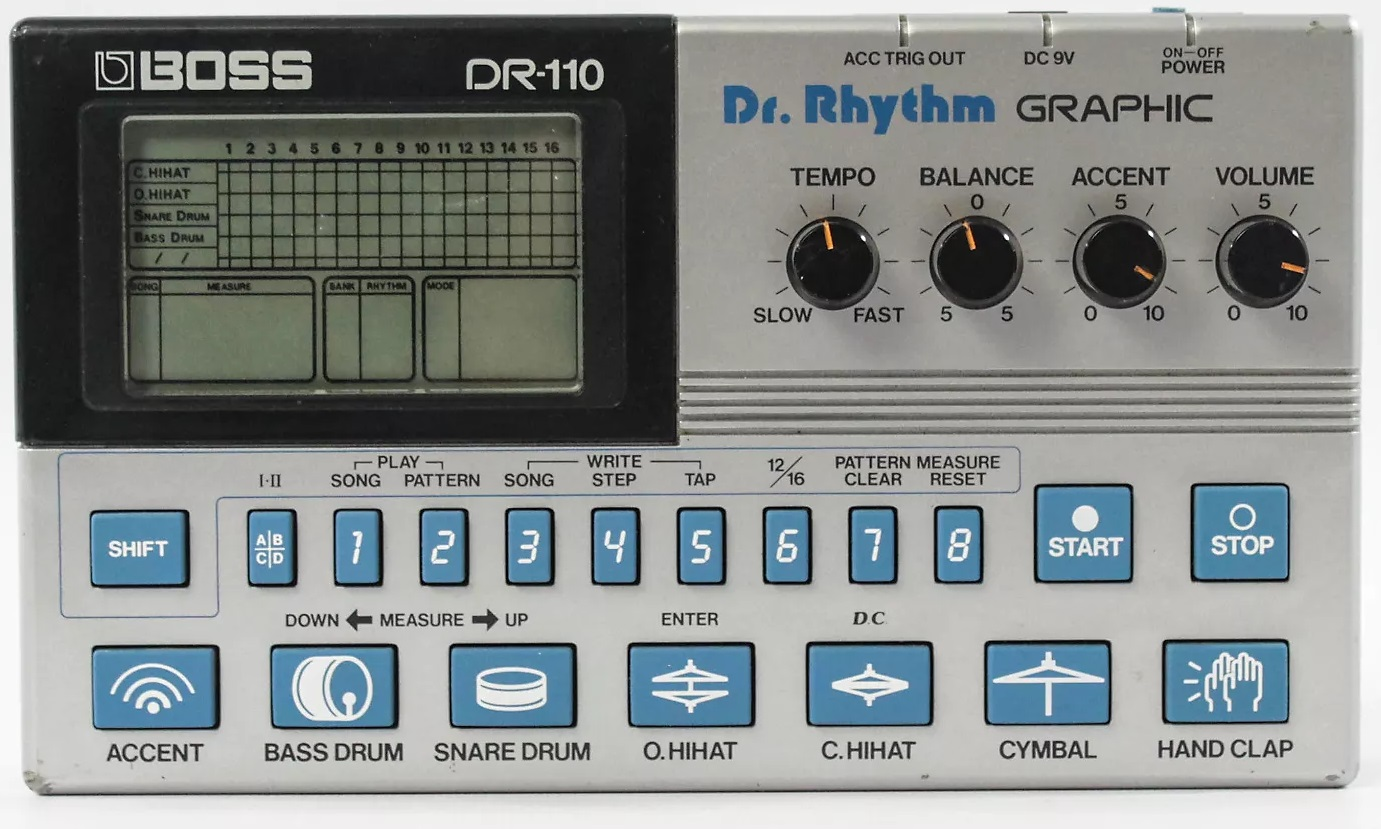
\includegraphics[width=6.9cm]{dr110}

The DR-110, the successor of the DR-55, has analogue sound but is programmed digitally using a LCD rhythm matrix. It quite possibly has the best analogue handclap ever. \\
\hline
LinnDrum & 1982 & 
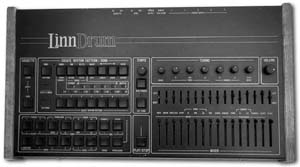
\includegraphics[width=8.4cm]{linndrum}

The LinnDrum originally sold for \$3,000 and about 5.000 units were produced. It provided the rhythm tracks of many 1980's hit records. \\
\hline
Rhythm Ace & 1973 & 
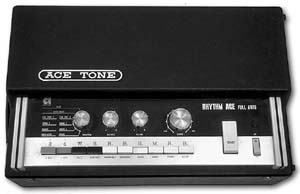
\includegraphics[width=6.2cm]{rhyace}

Ace Tone was the first company to produce electric rhythm boxes in Japan. In the UK, Bentley Pianos (who put stickers on all their products) distributed Ace Tone, and thus the machine is also known as the Bentley Rhythm Ace. \\
\hline
Tom \linebreak
Sequential \linebreak
Circuits & 1984 & 
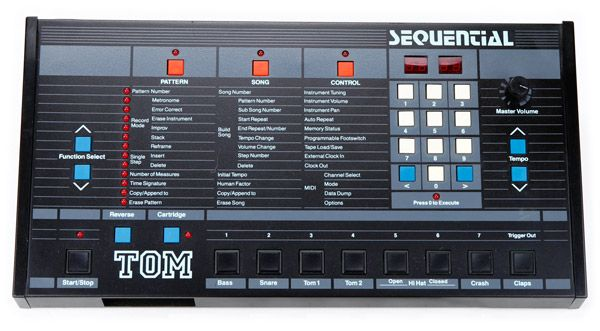
\includegraphics[width=8.0cm]{tom}

The sounds are a bit dirty and harsh sounding, especially next to its older brother Drumtraks, but that also gives Tom its character. The snare sounds like nothing else on this planet - it's electric! \\
\hline
Acieed House & 1990's & 

\includegraphics[width=3.6cm]{smiley_gray}

This set of vocal samples was derived from a bunch of popular Acid House tracks. Can you dig it? \\
\hline
Ghetto Bass & 1990's & 

\includegraphics[width=8.0cm]{booty} 

A bunch of samples derived from classic Detroit/Chicago ghetto house tracks.\\
\hline
Animals \linebreak Bud Melvin & 2004 & 

\includegraphics[width=8.0cm]{kit-farm} 

The winner of the 2004 Animal Sample Compo. A great selection of domestic animals. The Levi's 501 of animal kits! \\
\end{xtabular}

